\begin{slikaDesno}{fig/cim_rez.pdf}
    \textbf{\color{red}*}\PID
    У механичком систему са слике jе тег масе $m = 2\unit{kg}$ 
    обешен о опругу коефициjента
    еластичности $k = 8\unit{\dfrac Nm}$. 
    Опруга jе другим краjем фиксирана за ослонац коjи се може померати
    у вертикалном правцу. Отклон ослонца у односу на референтан положаj jе $x = x(t)$,
    а отклон тега \textit{у односу на равнотежни положај када је ослонац у 
    референтном положају} jе
    $y = y(t)$, као на слици. Побуда посматраног система jе $x$ а одзив jе $y$.
    Вектор гравитационог убрзања $\bf g$ усмерен је као на слици.
    \begin{enumerate}
        \item[(а)] Одредити функциjу преноса система, $H(s)$, у Лапласовом домену. 
    \end{enumerate}
\end{slikaDesno}
\begin{enumerate}
    \item[(б)] Применом Лапласове трансформације одредити
    принудни одзив овога система на побуду дату изразом
    $x(t) = X_{\rm m} (1 - \ee^{-\upsigma t}) \uu(t)$, где су 
    $\upsigma = 2 \unit{s^{-1}}$ и
    $X_{\rm m} = 5\unit{cm}$. 
    \item[(в)] Одредити и прелазни и устаљени одзив за задату побуду уколико је познато да је 
    $y(0^-) = 0$. 
\end{enumerate}

\textsc{\underline{Решење}}:
(а) Будући да је тег у равнотежном положају када је $x = y = 0$, то је сила гравитације уравнотежена тадашњим издужењем опруге. 
Према томе, на основу суперпозиције, те константне компоненте силе се се увек пократе, док преостаје додатна еластична сила
сила једнака $\Delta F_{\rm e} = k(x - y)$, референтно оријентисана навише. Једначина динамике система је стога 
\begin{equation}
    m \dfrac{\de^2 y}{\de t^2} = \Delta F_{\rm e} = k(x - y). 
\end{equation}
Преласком у Лапласов домен\footnote{Користи се особина $\LT{ \dfrac{\de x}{\de t} } = s \LT{x}$. } може се 
директно одредити функција преноса система као 
\begin{eqnarray}
    ms^2 Y(s) = k( X(s) - Y(s) ) 
    \Rightarrow
    H(s) = \dfrac{Y(s)}{X(s)} = \dfrac{k}{ms^2 + k} = \dfrac{\upomega_0^2}{s^2 + \upomega_0^2},
\end{eqnarray}
где је $\upomega_0 = \sqrt{\dfrac{k}{m}}$ природна (сопствена) учестаност посматраног система. 

(б) Лапласова трансформација побудног сигнала налази се таблично као 
\begin{equation}
    X(s) = \LT{ X_{\rm m} (1 - \ee^{-\upsigma t})\uu(t) } = X_{\rm m} 
    \left(
        \dfrac{1}{s} - \dfrac{1}{s + \upsigma}
    \right)
    =
    \upsigma X_{\rm m} 
        \dfrac{1}{s(s + \upsigma)}
\end{equation}
Лапласова трансформација одзива онда се може изразити као  
\begin{equation}
    Y(s) = H(s)\cdot X(s) = \upsigma \upomega_0^2 X_{\rm m} \dfrac{1}{s(s + \upsigma)(s^2 + \upomega_0^2)}
    = \upsigma \upomega_0^2 X_{\rm m} \dfrac{1}{s(s + \upsigma)(s + \jj\upomega_0)(s - \jj\upomega_0)}
\end{equation}
Растављањем на парцијалне разломке, коришћењем резултата из додатка \ref{a:pfd}, добија се израз облика
\begin{equation}
    Y(s) =  \upsigma \upomega_0^2 X_{\rm m} 
    \left(
        \dfrac{A_1}{s} + \dfrac{A_2}{s + \upsigma} + \dfrac{B}{s + \jj\upomega_0} + \dfrac{B^\ast}{s - \jj\upomega_0}
        \label{\ID.epfd}
    \right).
\end{equation}
Коефицијенте налазмо \textit{cover-up} методом: 
\begin{eqnarray}
    A_1 &=& \dfrac{1}{\xcancel{s}(s + \upsigma)(s^2 + \upomega_0^2)}\bigg|_{s = 0} 
        = \dfrac{1}{\upsigma \upomega_0^2} \\
    A_2 &=& \dfrac{1}{s\xcancel{(s + \upsigma)}(s^2 + \upomega_0^2)}\bigg|_{s = -\upsigma} 
        = - \dfrac{1}{\upsigma(\upsigma^2 + \upomega_0^2)} \\
    B   &=& \dfrac{1}{s(s + \upsigma)\xcancel{(s + \jj\upomega_0)}\underbrace{(s - \jj\upomega_0)}_{\jj2\upomega_0} } \bigg|_{s = - \jj\upomega_0 }
        =  -\dfrac{1}{2\upomega_0^2} \dfrac{1}{ (\upsigma - \jj\upomega_0)}
\end{eqnarray} 
Заменом добијених резултата у \eqref{\ID.epfd}, и применом инверзне Лапласове трансформације, даље се добија 
\begin{eqnarray}
    Y(s) &=& X_{\rm m} 
    \left(
        \dfrac{1}{s} 
        -
        \dfrac{\upomega_0^2}{\upomega_0^2 + \upsigma^2}
        \dfrac{1}{s + \upsigma}
        -
        \underbrace{
        \dfrac{1}{2}
        \dfrac{\upsigma}{\upsigma - \jj\upomega_0} 
        \dfrac{1}{s + \jj\upomega_0}
        -
        \dfrac{1}{2}
        \dfrac{\upsigma}{\upsigma + \jj\upomega_0} 
        \dfrac{1}{s - \jj\upomega_0}
        }_{\text{Видети и задатак \ref{z:damp_sin}}}
    \right) \\
    && \Downarrow \ILT{\bullet} \\ 
    y(t) &=&
    X_{\rm m}
    \left(
        1 
        -
        \dfrac{\upomega_0^2}{\upomega_0^2 + \upsigma^2} \ee^{-\upsigma t} 
        - \dfrac{\upsigma}{\sqrt{\upsigma^2 + \upomega_0^2}} 
        \cos\left(
            \upomega_0 t - \arctg\left( \dfrac{\upomega_0}{\upsigma} \right)
        \right)
    \right)
\end{eqnarray}
У конкретном случају задатих нумеричких вредности је  
$\upomega_0 = \upsigma = 2\unit{s^{-1}}$, па је онда 
\begin{equation}
    y(t) = 5 \left( 1 - \dfrac{1}{2} \ee^{-\upsigma t} - \dfrac{1}{\sqrt 2} \cos\left(\upomega_0 t - \dfrac{\uppi}{4} \right) \right) \, \uu(t) \unit{cm}
\end{equation}
На слици \ref{fig:\ID.rez} приказан је временски дијаграм добијеног резултата. На истој слици приказани су 
задата побуда и одређени одзив система.

\begin{figure}[ht!]
    \centering
    \begin{subfigure}{0.49\textwidth}
        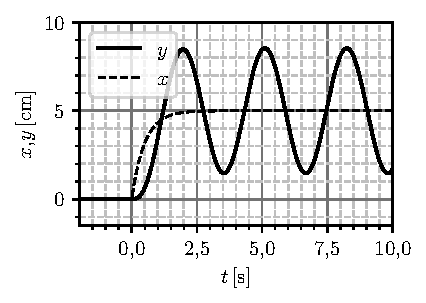
\includegraphics{fig/cim_rez_plot.pdf}
        \caption{Временски дијаграм комплетног одзива}
        \label{fig:\ID.rez}    
    \end{subfigure}
    %
    \begin{subfigure}{0.49\textwidth}
        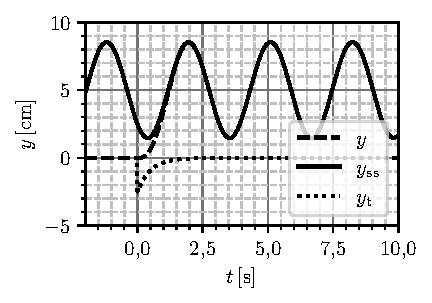
\includegraphics{fig/cim_rez_razni_plot.pdf}
        \caption{Различите врсте одзива}
        \label{fig:\ID.rez2}    
    \end{subfigure}
\end{figure}

(в) Устаљени одзив система представљају стална и простопериодична компонента, 
$y_{\rm ss} = 5 - \dfrac{5}{\sqrt 2} \cos\left(\upomega_0 t - \dfrac{\uppi}{4} \right) \unit{cm}.$, док 
прелазни одзив представља преостао експоненцијални члан 
$y_{\rm t} = - \dfrac{5}{2} \ee^{-\upsigma t} \uu(t) \unit{cm}$. Упоредни приказ свих врста одзива 
приказан је на слици \ref{fig:\ID.rez2}.